\chapter{Canonical products and their conjugate diagrams}\label{chap10}%chap 10

\section{Canonical products and location of conjugate
  diagram}\label{chap10:sec1} %sec 1

Given\pageoriginale a sequence $\Lambda = \{\lambda_n\}, \big|\lambda_n \big| \to
\infty$, it is always possible to construct an entire function with
$\lambda_n$ as zeros. We suppose $\Lambda$ to be symmetric, $\Lambda =
\{\pm \lambda_n\}, \big|\lambda_{n + 1} \big| \ge \big| \lambda_n
\big| (n = 1,2, \ldots ), \sum\limits^{\infty}_{1}
\dfrac{1}{|\lambda_n|^2} < \infty$, and (to avoid complications),
$|\lambda_1| > 0$. Then the simplest of these functions is the
canonical product 
$$
C(w) = \prod^\infty_1 \left(1 - \frac{w^2} {\lambda_n 2}\right).
$$

For example, if $\lambda_n = n, C(w) = \dfrac{\sin \pi w}{\pi
 w}$. With convenient hypothesis about the $\lambda_n$, we shall see
that $C(w)$ is an entire function of exponential type, and be able to
locate its conjugate diagram. 

We first recall the following definitions (Mandelbrojt $2$).
\begin{align*}
 n(r) & = \sum_{|\lambda n | < r} 1 : \text { distribution function
  of } \Lambda.\\ 
 D(r) & = n (r) / r : \text { density function of } \Lambda.\\
 D^. &= \lim \sup\limits_{r \to \infty} D(r) : \text{ upper density
  of } \Lambda.\\ 
 D. &= \lim \inf_{r \to \infty} D(r) : \text{ lower density of } \Lambda.
\end{align*}

We have $D., = \lim \sum \dfrac{n}{|\lambda n|} \ge \lim \inf
\dfrac{n}{|\lambda n|} = D. ~ $. When $D^. = D = D$,. we define 
$D$ to be the density of $\Lambda$. 

$\bar{D}(r) = \dfrac{1}{r} \int^r_o D(t) dt :$ Mean density function
of $\Lambda$. 

We define the mean upper density $\bar{D}^{.}$, mean lower density
$\bar{D}$., and the mean density $\bar{D}$ in the same way. We have
$D. \le \bar{D}. \le \bar{D} \le D^{.}$, and one can prove $D^. < e
\bar{D}^{.}$ (Mandelbrojt $3$). 

\medskip
\noindent
\textbf{Calculation\pageoriginale of Mandelbrojt (Mandelbrojt $3$) . .}

We make the hypothesis that $\bar{D}^{.} < \infty$, and we majorise
the type of $C(w)$, in order to have a location of the conjugate
diagram. 
$$
\big| C(w) \big| \le \prod \left(1 + \frac{r^2}{|\lambda|^2}\right) =
\varphi (r), \log \varphi (r) = \int^\infty_o \log \left(1 +
\frac{r^2}{|\lambda_n|}\right) dn (\lambda). 
$$

To calculate $\varphi(r)$ we integrate by parts
$$
\int^x_o \log (1 + {r^2}{|\lambda^2|}) dn (\lambda) = \int^x_o \frac{n
 (\lambda)}{r^2 + \lambda^2} \frac{n (\lambda)}{\lambda} d \lambda +
 \left[n (\lambda) \log \left(1 + \frac{r^2}{\lambda 2}\right)\right]^x_o. 
$$

Since $\bar{D}^{.} < \infty$, we cannot have $\dfrac{n(X)}{X} \to
\infty$. Therefore there exists a sequence $X_n \to \infty$, such that
$\dfrac{n (X_n)}{x^2_n} \to 0$. Since $n (0) = 0$ and 
$$
\displaylines{\hfill 
n(x_n) \log \left(1 + \frac{r^2}{x^2_n}\right) \to 0 \text{ as } x_n
\to \infty \hfill \cr
\text{we have}\hfill 
\log \varphi(r) = \int^\infty_o \frac{2r^2}{r^2 + \lambda^2}
d(\lambda ) D \lambda. \hfill \cr
\hfill \int^x_o \frac{2r^2}{r^2 + \lambda^2} D ( \lambda ) d \lambda =
\int^x_o \frac{4r^2}{(r^2 + \lambda^2)^2} \lambda \bar{D} (\lambda) d
\lambda + \left[\lambda \bar{D} (\lambda) \frac{2r^2}{r^2 +
 \lambda^2}\right]^x_o. \hfill }
$$

So,
\begin{gather*}
 \log \varphi (r) = \int^\infty_o \frac{4r^2 \lambda^2}{(r^2 +
 \lambda^2)^2} \bar{D} (\lambda) d \lambda = r \int^\infty_o
 \frac{4t^2}{(1 + t^2)^2} \bar{D} (t_r) dt.\\ 
 \lim \sup_{r \to \infty} \frac{\log \varphi (r)}{r} \le \bar{D}^{.}
 \int^\infty_{0} \frac{4t^2}{(1 + t^2)^2} dt. 
\end{gather*}

We have $\pi = \int\limits^{\infty}_{o} \dfrac{4t^2}{(1 +
 t^2)^2}dt$. This gives the relation 
$$
\underline{ \underline{h (\theta) \le \pi \bar{D}^{.}}} \qquad (M)
$$

Geometrically, this signifies that the conjugate diagram is situated
in a circle with centre at origin and or radius $\pi \bar{D}^{.}$. 

\medskip
\noindent
\textbf{Calculation of Carlson (Bernstein, note $III$).}

We now suppose that we have one of the following equivalent relations
$$
\big[ D^{.} = D_.= D = 1, \arg \lambda_n \to 0 \Longleftrightarrow
 \frac{\lambda n} {n} \to 1.\big] 
$$ 

Under\pageoriginale these conditions the conjugate diagram is particularly
simple. Suppose $\lambda_n = n$. Then $C(w) = \dfrac{sin \pi w}{\pi
 w}$ is of type $\pi$ in the upper and lower half planes. Also we
have $h(0) = h(\pi) = 0$. Since the conjugate diagram is convex, it is
the segment between $\pi i$ and $- \pi i$. 

Now,
$$
\frac{\pi w C(w)}{\sin \pi w} = \prod \frac{(1 - w^2 /
 \lambda^2_n)}{(1 - w^2 / n^2)} = \prod \left(1 + \frac{w^2/n^2 - w^2 /
 \lambda^2_n}{1 - w^2 / n^2}\right). 
$$

Let $0 < \alpha < \dfrac{\pi}{4}$, and $w = r e^i \theta, \alpha <
|\theta| < \dfrac{\pi}{2}$. In this case, we have the inequality $|w^2
- n^2| > n^2$ sin $2 \alpha$. Since $(\lambda^2_n - n^2) / \lambda^2_n
\rightarrow 0$, we have the following inequalities: 
\begin{align*}
 \bigg |\frac{\pi w C(w)}{\sin \pi w}\bigg | & \le \prod^\infty_1 \left| 1
 + \frac{w^2(\lambda^2_n - n^2) / \lambda^2_n}{n^2 - w^2}\right| =
 \prod^\infty_1 X_n \\ 
 & \prod^{N-1}_1 X_n \prod^\infty_N (1 + \frac {\varepsilon r^2}{n^2
 \sin 2 \alpha}) \\ 
 & \prod^{N-1}_1 X_n |\sin (i \pi r \sqrt{\varepsilon / \sin 2\alpha})|
\end{align*}

This gives us $ \limsup \limits_{r \rightarrow \infty} 1 / r \log
\dfrac {C(w)}{\sin \pi w} \le 0$; from which we have 
$$
\limsup \limits_{r \rightarrow \infty} \frac{\log|C(w)|}{r} \le \pi
|\sin \theta |, \theta \neq 0, \pi (\mod 2 \pi) 
$$ 

By taking the function $(\sin \pi w) / \pi w C(w)$ we have the same
calculation with the roles of $\lambda_n$ and $n$ interchanged. Since
$\dfrac{n}{\lambda_n} \rightarrow 1$, we can replace $\lambda_n$ by
$n$ for large values of $n$ in majorising $(\sin \pi w)/ \pi w C(w)$
and get the reverse inequality. Thus we get 

$(c)$ $\limsup \limits_{r \rightarrow \infty} | \dfrac{\log C(w)}{r}| =
\pi |\sin \theta |, w = r e^{i \theta}, \theta \neq 0, \pi (\mod 2
\pi)$. This result shows us that if the density of $\Lambda$ is $D$,
then the conjugate diagram of $C(w)$ is the segment joining $i \pi D$
and $-i \pi D$ 
\medskip
\pageoriginale

\noindent 
\begin{minipage}[c]{5.8cm}
\quad We can relax slightly the hypothesis in the calculation of Carlson,
viz., make the hypothesis that $D = 1$ and $\lim \sup | arg \lambda_n
| \le \alpha \le \dfrac{\pi}{2}$. Then, for $n > N, |arg \lambda_n| <
\alpha + \varepsilon = \alpha$. Taking $0 < arg w = < \frac{\pi}{2} -
\alpha'$ we have 
$$
\prod^\infty_N \bigg |1- \frac{w^2}{\lambda_{n^2}} \bigg| <
\prod^\infty_N \bigg | -1 \frac {w^2}{\lambda_n^2 e^{- 2i
 \alpha'}}\bigg |. 
$$
Hence $h(\theta) \le \pi sin (\pi + \alpha)$ if $0 < \theta < \pi/2 -
\alpha'$.In this case the conjugate diagram turns out to be contained
in the portion of the disc $|z| \le \pi$, containing $0$ and bounded
by the lines $x = \pm \pi \sin \alpha$. 
\end{minipage}
\begin{minipage}[c]{5cm}
\begin{figure}[H]
\centerline{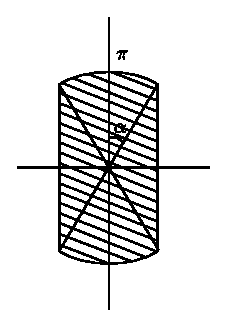
\includegraphics{vol15-figures/fig15-3.eps}}
\end{figure}
\end{minipage}

\section{Theorems of Jensen and Carleman}\label{chap10:sec2}%Sec

We now recall well - known formulae which will be used in the problems
of closure and quasi- analyticity among others. 

\noindent
\textbf{Jensen's formula.} \textit{Let $F(w)$ be a function
 meromorphic inside and continuous on a circle of radius $R$ and
 center $0$, and let $F(w)$ be without zero or pole at $0$ and on
 $|w|= R$. Denote by $n_1(r)$ the number of zero in $|z| < r$ and by
 $n_2(r)$ the number of poles in $|z| < r$. Then we have the
 following relation: } 
$$
\int^R_0 \left( \frac{n_1(r)}{r} - \frac{n_2(r)}{r} \right) dr =
\frac{1}{2\pi} \int^{2 \pi}_{0} log \frac{F(Re^{i \theta})}{F(0)}d 
$$
\textbf{Carleman's formula.} \textit{Let $F(w)$ be meromorphic in the
 half plane $u \ge 0 (w = u+ iv)$ with zeros at $r_k e^{i \theta_k}$
 and poles at $\varrho_j e^{i \alpha_j}$ and with no zero or pole on
 $u = 0$. Taking a contour $D$ consisting of a part of the imaginary
 axis and a semi - circle of radius $R$ and center $0$ in the half
 plane\pageoriginale $u \ge 0$, we have the following relation:} 
\begin{align*}
&\sum \left(\dfrac{1}{r_k} - \dfrac{r_k}{R^2}\right) \cos \theta_k
-\left(\dfrac{1}{\rho_j}- \dfrac{\rho_j}{R^2}\right) \cos \alpha_j\\ 
&\qquad=\dfrac{1}{\pi R} \int\limits^{\pi /2}_{\pi /2} \log |F (Re^{i \theta})| \cos
\theta d \theta\\ 
&\qquad\quad+ \dfrac{1}{2 \pi} \int^R_0 \left(\dfrac{1}{y^2} -
\dfrac{1}{R^2}\right) \log |F(iy) F(-iy)| dy + 0(1)
\end{align*}

the summation being on $r_k e^{i \theta k}, \rho_j e^{i \alpha_j}$ inside $D$.

For the proofs $Cf$. Titchmarsh.
